\documentclass[tikz,border=10pt]{standalone}
\usetikzlibrary{arrows,automata}

\begin{document}
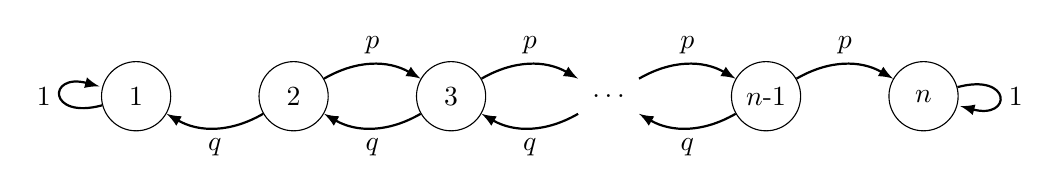
\begin{tikzpicture}[node distance=2cm,->,>=latex,auto,
  every edge/.append style={thick}]
  \node[state] (1) {$\rm 1$};
  \node[state] (2) [right of=1] {$\rm 2$}; 
  \node[state] (3) [right of=2] {$\rm 3$};
  \node (4) [right of=3] {$\ldots$};
  \node[state,opacity=0] (4) [right of=3] {$\ldots$};
  \node[state] (5) [right of=4] {$n$-$1$};
  \node[state] (6) [right of=5] {$n$};
  \path (1) edge[loop left] node{$1$} (1);
  % \path (1) edge[bend left] node{$p$} (2);
  \path (2) edge[bend left] node{$q$} (1);
  \path (2) edge[bend left] node{$p$} (3);
  \path (3) edge[bend left] node{$q$} (2);
  \path (3) edge[bend left] node{$p$} (4);
  \path (4) edge[bend left] node{$q$} (3);
  \path (4) edge[bend left] node{$p$} (5);
  \path (5) edge[bend left] node{$q$} (4);
  \path (5) edge[bend left] node{$p$} (6);
  % \path (6) edge[bend left] node{$q$} (5);
  \path (6) edge[loop right] node{$1$} (6);
\end{tikzpicture}
\end{document}

